\documentclass[10pt]{beamer}

\usetheme{metropolis}
\usepackage{appendixnumberbeamer}

\usepackage{booktabs}
\usepackage[scale=2]{ccicons}

\usepackage{tikz}
\usetikzlibrary{arrows,automata}

\usepackage{pgfplots}
\usepgfplotslibrary{dateplot}


\PassOptionsToPackage{table}{xcolor}
\usepackage{colortbl}

\usepackage{xspace}
\newcommand{\themename}{\textbf{\textsc{metropolis}}\xspace}

\title{RoboCup - System}
%\subtitle{A modern beamer theme}
\date{October 26, 2017}
\author{Florian Lier \& Johannes Kummert \& Dominik Sixt}
%\institute{Center for modern beamer themes}
%\titlegraphic{\hfill
\includegraphics[height=1.5cm]{logo.pdf}}
\titlegraphic{\hfill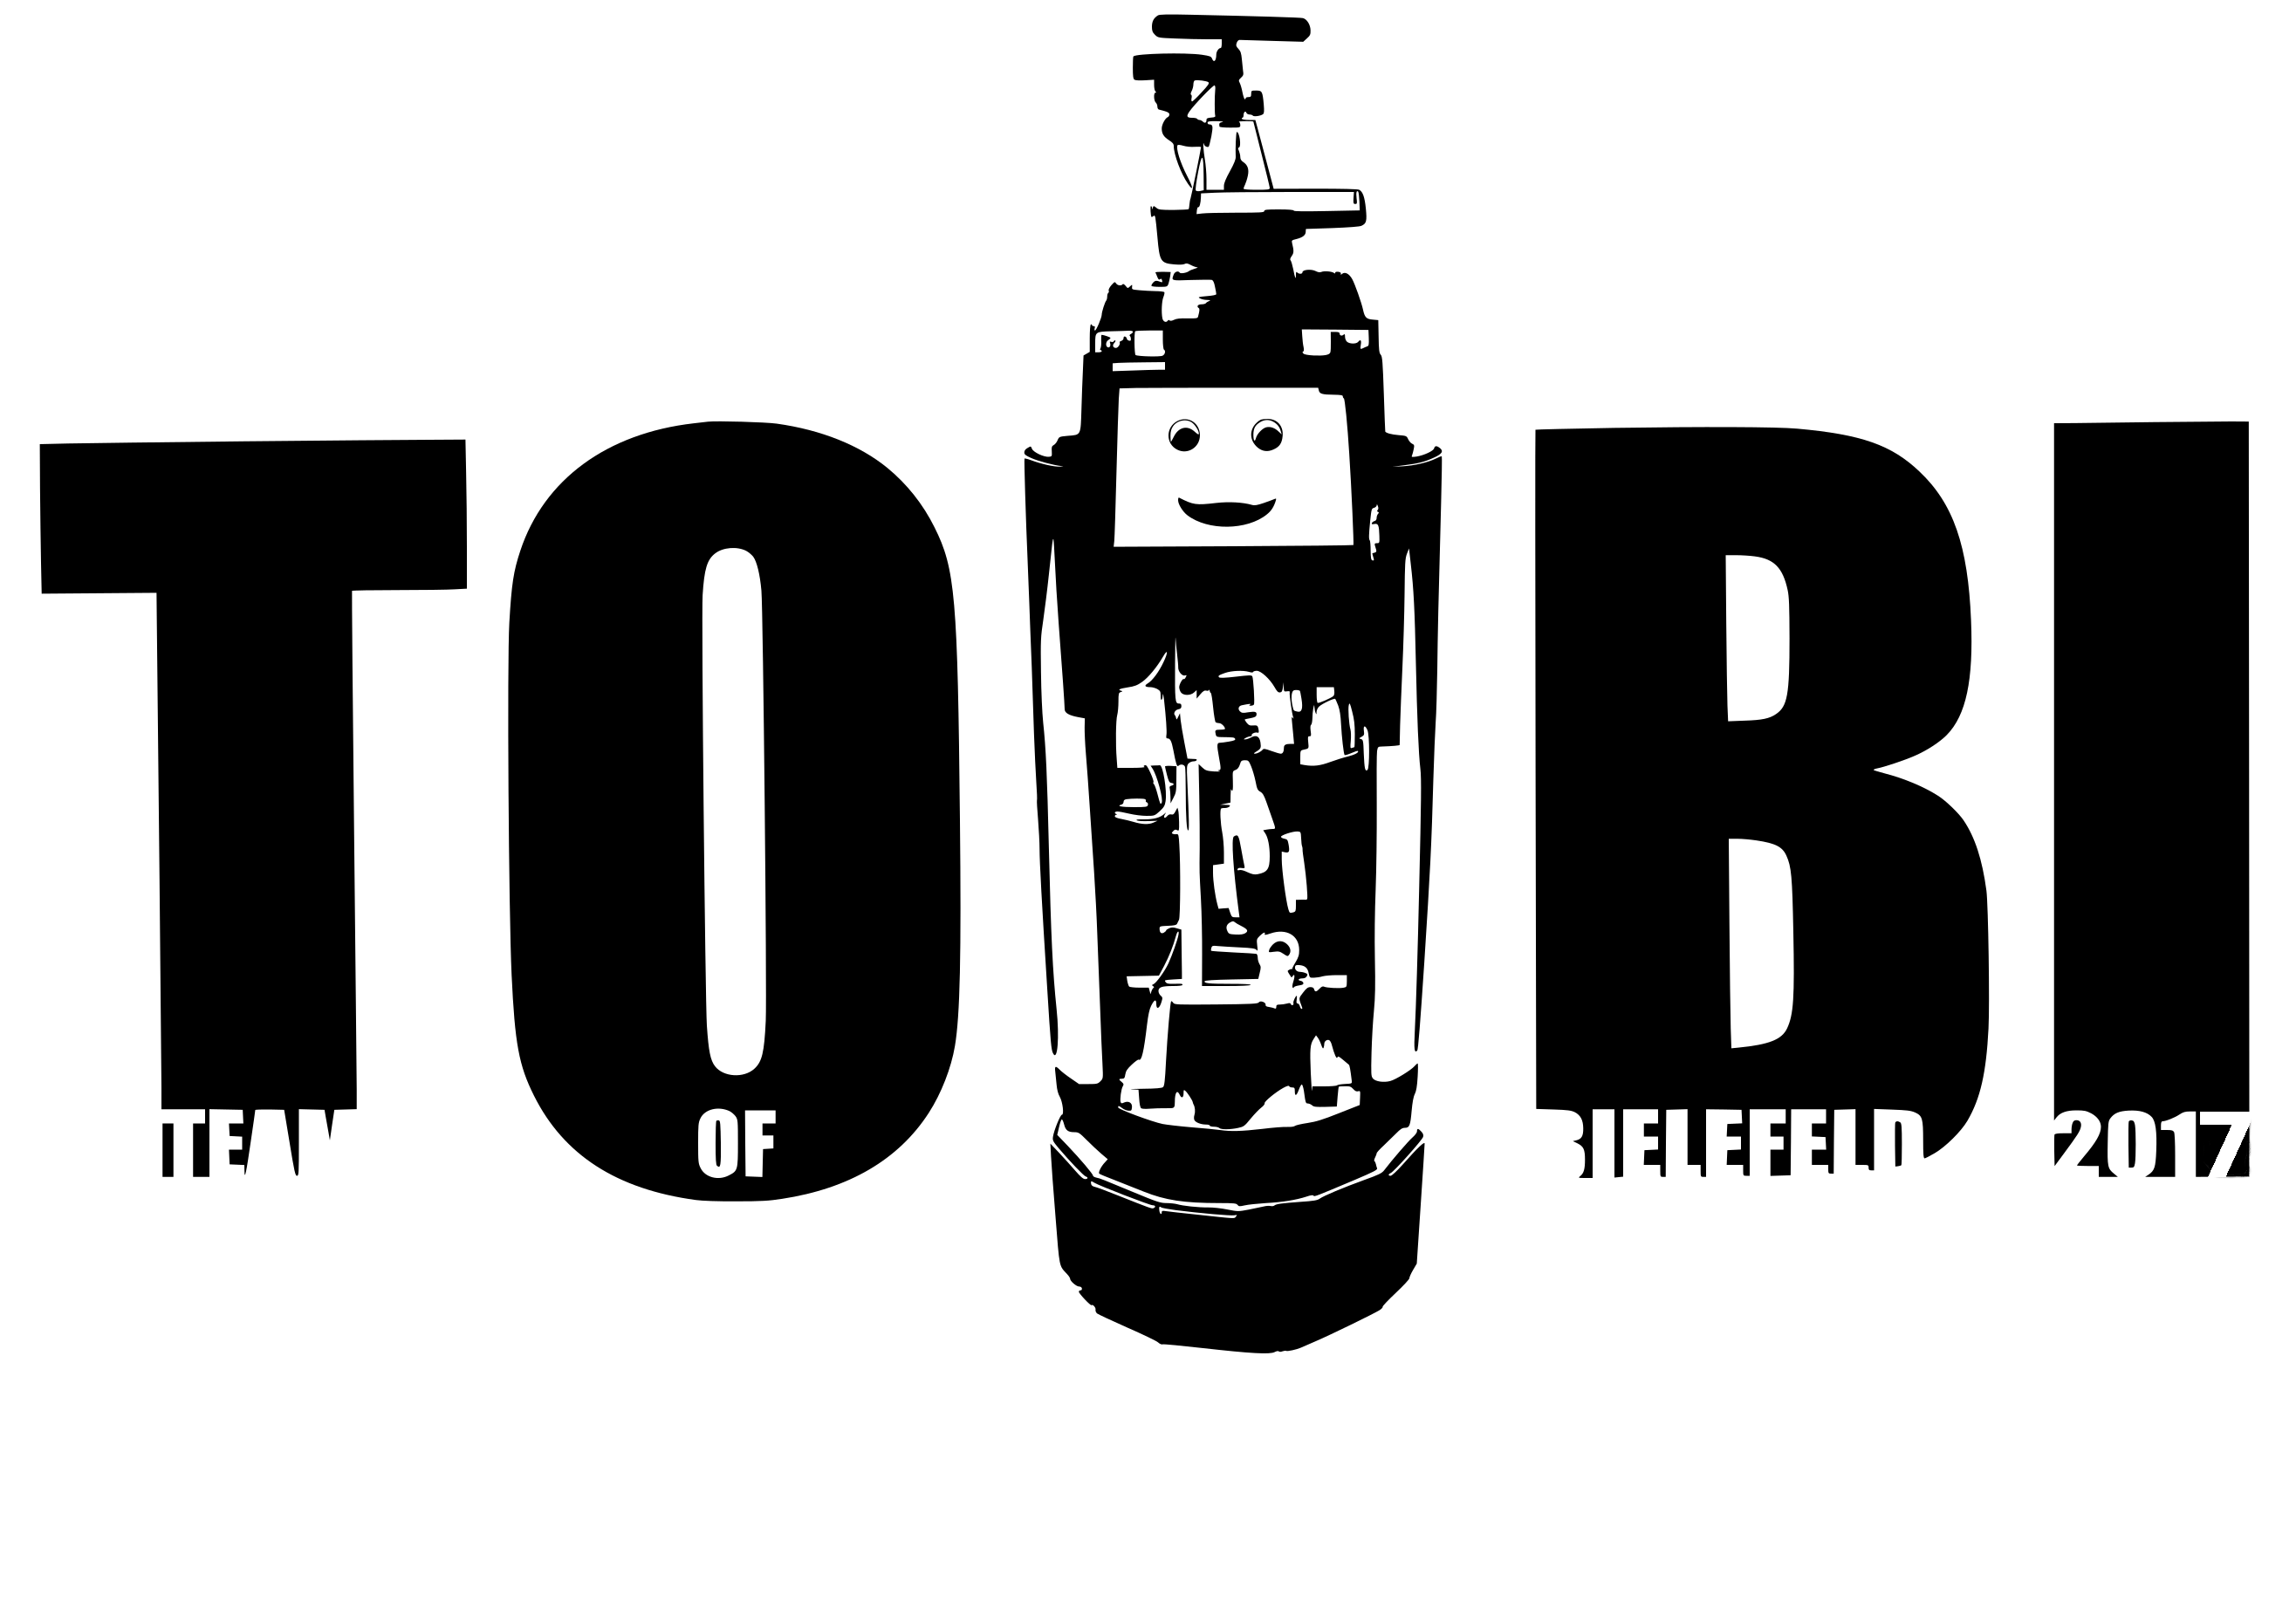
\includegraphics[height=1.5cm]{tobi_logo.png}}

\begin{document}

\maketitle

\begin{frame}{Table of contents}
  \setbeamertemplate{section in toc}[sections numbered]
  \tableofcontents[hideallsubsections]
\end{frame}

\section{Cognitive Interaction Toolkit}

\begin{frame}[fragile]{Motivation}
	

\end{frame}

\begin{frame}[fragile]{Concept}
	
	
\end{frame}

\section{vDemo}

\begin{frame}[fragile]{Motivation}
	\alert{What is vDemo and why should we use it?}
	\begin{itemize}
		\item distributed system with several computing machines
		\item advanced overview % handling of all components
		\item controlling and debugging % stop, check etc. // for debugging
		\item individual component configuration 
	\end{itemize}
	
	
\end{frame}

\begin{frame}[fragile]{Overview}
	% For each Task a Script .sh.in
	% Each component for a application
	% Components organized in Tabs
	
	\begin{figure}
		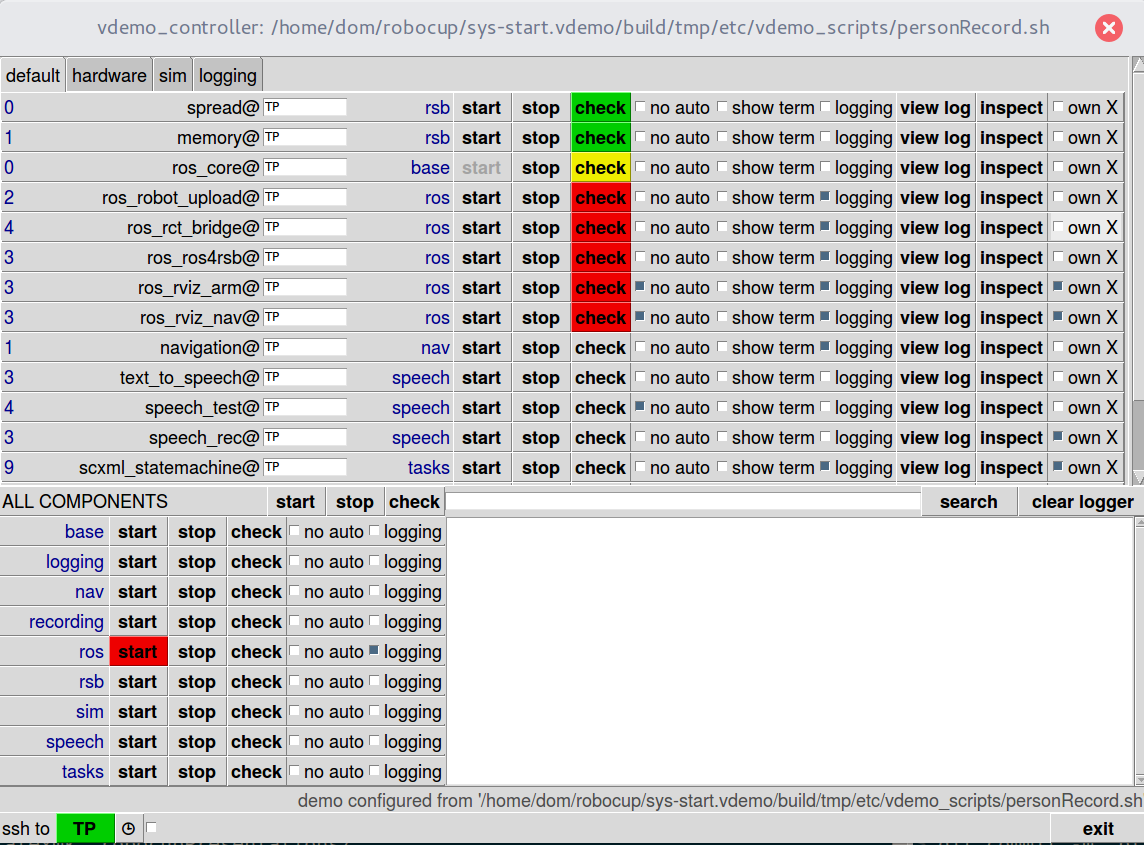
\includegraphics[scale=0.185]{vdemo_overview.png}
		\caption{Example of a started vDemo.}
	\end{figure}
	%TODO: New Picture
	
\end{frame}


\begin{frame}[fragile]{Arrangement of vDemo}
	\begin{itemize}
		\item \alert{Groups}: To group related components and to enable start of all included components
	\item \alert{Level}: To start components in proper order 
	\item \alert{Tabs}: To organize a plenty of components more clearly
	\item \alert{Start / Stop / Check}: To handle each component and get status information
	\item \alert{Checkboxes}: To activate autostart and logging
	\end{itemize}
\end{frame}

\begin{frame}[fragile]{Component indicator colors}
	\alert{Components might be running independently from vdemo} % no screen process is present
	\begin{center}
		
		\begin{figure}
			
			
			\begin{tabular}{|l|l|}
				\hline
				\cellcolor{gray!50}check & unknown \\
				\hline
				\cellcolor{yellow}check & starting \\
				\hline
				\cellcolor{green}check & running + responding \\
				\hline
				\cellcolor{orange}check & responding, but not started from vdemo \\
				\hline
				\cellcolor{pink}check & running, but not responding \\
				\hline
				\cellcolor{red}check & not running \\
				\hline
			\end{tabular}
			\caption{Color indicator of components}
		\end{figure}
	\end{center}
\end{frame}

\begin{frame}[fragile]{Structure of vDemo Script}
	\alert{}
	
	\begin{center}
		\begin{figure}
		
		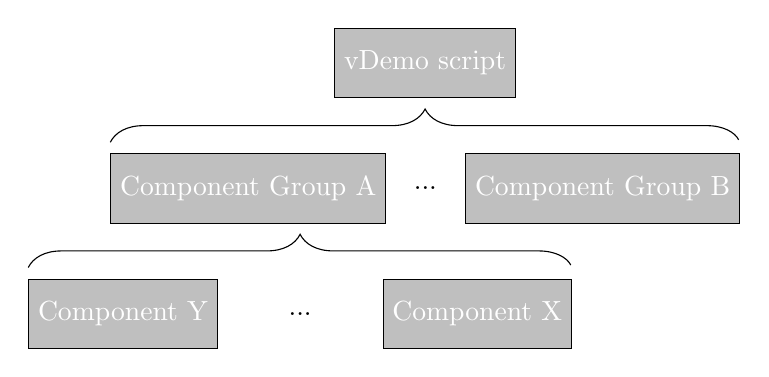
\begin{tikzpicture}[->,>=stealth',shorten >=1pt,auto,node distance=2.25cm,
		thin]
		\tikzstyle{every state}=[fill={rgb:black,1;white,3},draw=black,text=white,minimum width=1.5cm, rectangle]
		%\tikzset{every loop/.style={min distance=10mm,in=-5,out=10,looseness=15}}
		
		\node[state]	(MidA)              			        {Component Group A}; 
		\node[]    		(MidDots) 	[right of=MidA] 			{...};
		\node[state]    (MidB) 		[right of=MidDots] 			{Component Group B};
		\node[state]    (BottomA) 	[below left of=MidA] 		{Component Y};
		\node[]    		(BottomDots)[right of=BottomA] 			{...};
		\node[state]    (BottomB) 	[right of=BottomDots] 		{Component X};
		
		%\node [above of=O, font=\large, node distance=2cm] (titleOperator) {\underline{Give Commands}};
		
		%\path 
		%(B) edge              											node {detect obstacle} (C)
		%(B) edge   		[loop below]						            node {self diagnosis} (B)
		%(O) edge   		[bend right=5, align=center,swap]		            node {commanding} (B)
		%(B) edge   		[bend right=5, align=center, swap]              node {repeating} (O)
		%(B) edge   		[bend left=5, align=center]		     	  	    node {feedback\\procedures} (P)
		%(P) edge   		[bend left=5, align=center]						node {feedback in\\offering selection} (B)
		%(O) edge 		[bend right=5] 									node {} (P)
		%;
		
		\draw[-,decorate,decoration={brace,amplitude=12pt,raise=4pt}] (MidA.north west)
		-- (MidB.north east) node [state,midway,yshift=20pt]{vDemo script} ; % vdemo master shell script
		\draw[-,decorate,decoration={brace,amplitude=12pt,raise=4pt},xshift=20pt] (BottomA.north west)
		-- (BottomB.north east);
		\end{tikzpicture}
		\caption{Components are summarized in groups which are included in the master vDemo script.}
	\end{figure}
	\end{center}
\end{frame}

\begin{frame}[fragile]{Component}
	\begin{itemize}
		\item shell script with predefined functions
		\item executes desired software in own shell environment % loaded own .bashrc + vdemo shell master script arguments + exported variables
	\end{itemize}
	
	\alert{Component Functions} %To customize the behaviours
	\begin{itemize}
		\item \texttt{start\_component}
		\item \texttt{stop\_component}
		\item \texttt{on\_stop}
		\item \texttt{on\_check}
	\end{itemize}
	
	
\end{frame}







\section{BonSAI} % ... Sensor Actuator Interface
\begin{frame}[fragile]{BonSAI - Motivation}
	
	\begin{itemize}
		\item multiple software components
		\item perception and interpretation
		\item complex scenarios
		\item component agnostic
		\item robot agnostic
	\end{itemize}
	
\end{frame}

\begin{frame}[fragile]{BonSAI - Layers}

	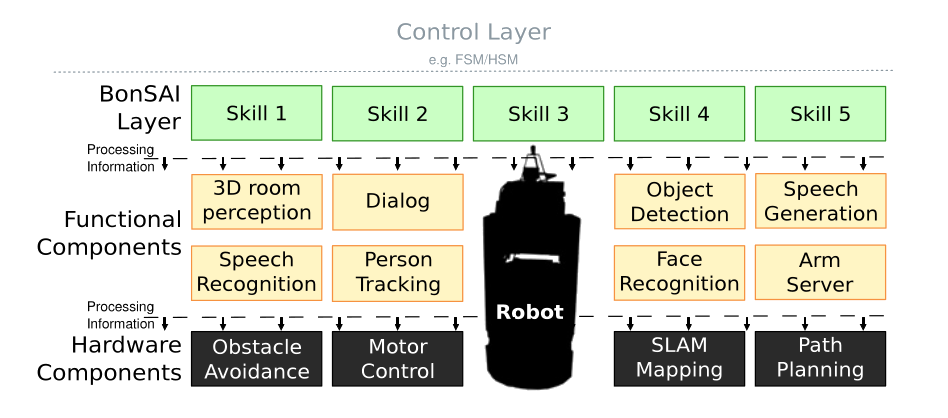
\includegraphics[scale=0.35]{bonsai_layerCut}

\end{frame}

\begin{frame}[fragile]{BonSAI - Structure}
	
	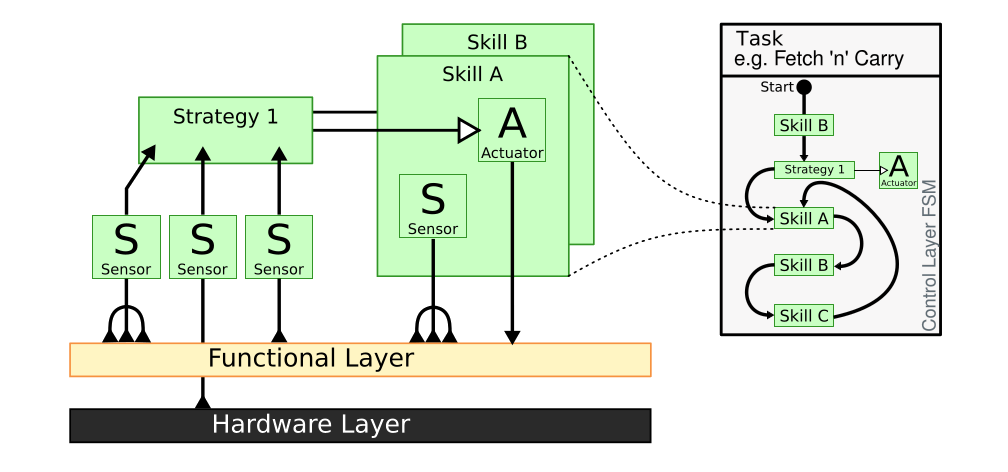
\includegraphics[scale=0.32]{bonsai_usageCut}
	
\end{frame}

\begin{frame}[fragile]{BonSAI - Example}
	
	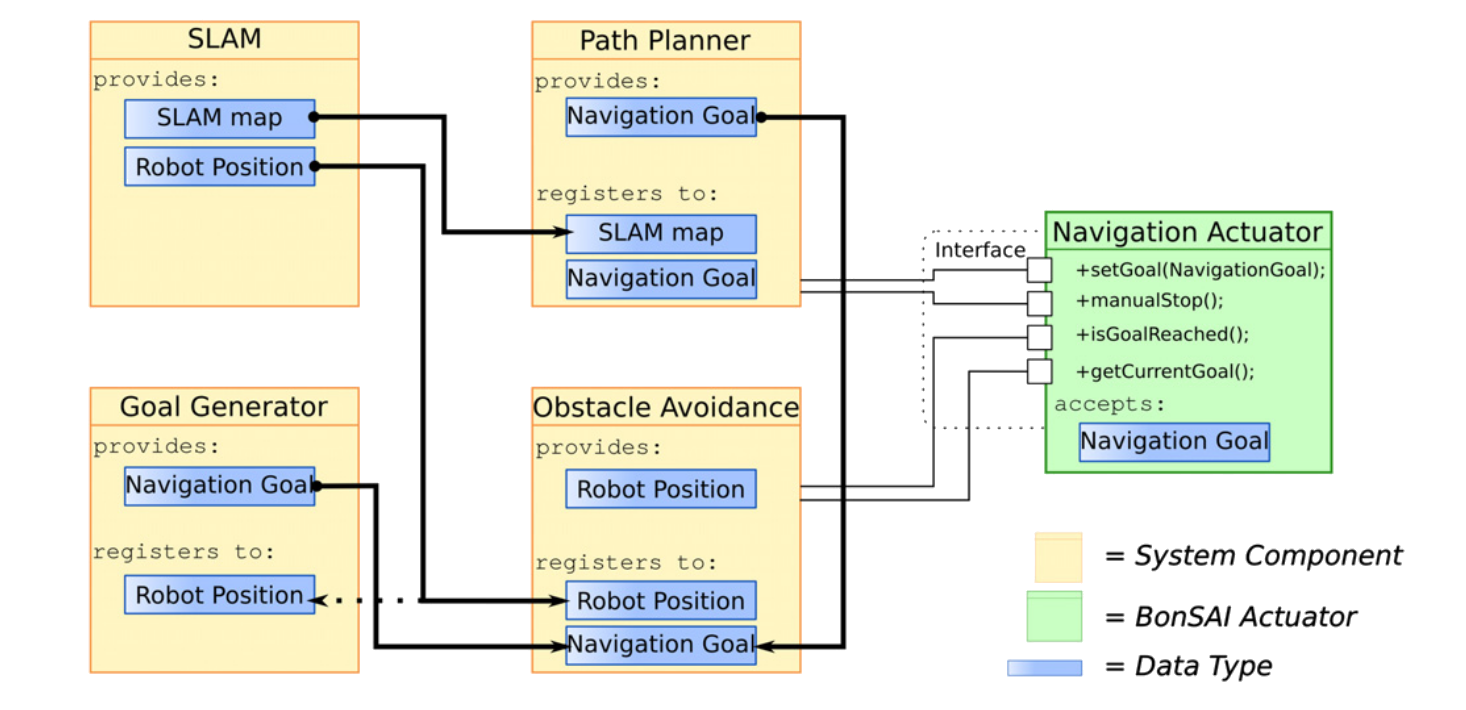
\includegraphics[scale=0.23]{bonsai_navCut}
	
\end{frame}

\begin{frame}[fragile]{Metropolis}

  The \themename theme is a Beamer theme with minimal visual noise
  inspired by the \href{https://github.com/hsrmbeamertheme/hsrmbeamertheme}{\textsc{hsrm} Beamer
  Theme} by Benjamin Weiss.

  Enable the theme by loading

  \begin{verbatim}    \documentclass{beamer}
    \usetheme{metropolis}\end{verbatim}

  Note, that you have to have Mozilla's \emph{Fira Sans} font and XeTeX
  installed to enjoy this wonderful typography.
\end{frame}


\begin{frame}[allowframebreaks]{References}

  \bibliography{demo}
  \bibliographystyle{abbrv}

\end{frame}

\end{document}
